\documentclass[a4paper, 12pts]{article}

\usepackage[top=3.5cm, bottom=3.5cm, left=3cm, right=3cm]{geometry}

\usepackage[T1]{fontenc}
\usepackage[utf8]{inputenc}
\usepackage[french]{babel}
\usepackage{textcomp}
\usepackage{listings}
\usepackage{authblk} %author tools
\usepackage{enumitem}
\usepackage{amssymb}
\usepackage{graphicx}

%\usepackage{hyperref} %pour les liens internet

%\usepackage{graphicx} %pour les images
\title{TP C++ n°3 : Analyse de logs Apache}
\author{Edern HAUMONT}
\author{Nicolas SIX}
\affil{B3111}
\date{\today}

%-----------------------------------------------------------------------------------------


\begin{document}

%\begin{titlepage}

\maketitle

%\end{titlepage}

%----------------------------------------------Title end

\section{Specifications}
\subsection{General specifications}
\paragraph{}
 Our program is designed to deal with apache servers log files.

The input of our program (analog) is a correctly built (cf. detailed specs) log file (.log). The output is the list of the ten most visited URL on the server. This list is printed on the standard output. Some options are available to detail the request. The program is able to generate a .dot file which may be viewed with Softwares like Graphviz.
 The program is made to deal quickly with big to be easily updated if the treatment needs of the user evolve.log files. However, it is designed to be easily updated if the treatment needs of the user evolve. That is, if someone wants to modify the application to add a classification level to the Data structure, it must be easy for him/her. The users should not be a programmer, simply a server administrator.
 The program is designed for linux systems.

\subsection{Log lines}
\paragraph{}
 A log line must fulfill several conditions in order to be accepted by the program. Besides the conditions on each information, there is a general structure to check :
 \begin{itemize}[label=$\square$]
 \item there is a specific order for the informations in a logline
 \item each information in seperated from the others with a space. However, the request, the referrer, and browser informations are given between double quotes.
 \end{itemize}
 Each information of a log line is the object of a small test.
 \begin{itemize}[label=$\square$]
 \item Ipv4 adress. The program does not check its validity. test : TestIpv4
 \item User logname. It must be in one world. If there is none, it is replaced by a dash ("-"). test : TestPseudo\&Logname
 \item Authenticated User (Pseudo). It must be in one world. If there is none, it is replaced by a dash ("-"). test : TestPseudo\&Logname
 \item Date, time and GMT as followed : [DD/Mon/YYYY:HH:MM:SS XGMT] (X replaced by "+" or "-"). test : TestDate\&hour\&GMT

 these conditions may be added
 \begin{itemize}
 \item date < current date
 \item hour between 00:00:00 and 23:59:59
 \item GMT between -12 and +12
 \end{itemize}
 \item Total request as followed (no constraint of world size) : "REQUESTTYPE requestedURL requestProtocol" . The only request that must be considered as valid by the program is GET, the other are accepted but not treated. tests : TestRequestType, TestRequestDestination, TestRequestProtocol
 \item Return code between 100 and 400, codes above 300 included are considered as fail codes. test : TestReturnCode
 \item Size of transmission >= 0. If it is unknown, it is replaced by a dash ("-"). test : TestDataSize
 \item Referrer. It is given between double quotes. test : TestReferrer
 \item Browser and browser infos given between double quotes. test : TestBrowser
 \end{itemize}
\paragraph{}
 Here is a log line template given as example :

 MyIpAdress Logname Pseudo [DD/Mon/YYYY:HH:MM:SS XGMT] "REQUESTTYPE requestedURL requestProtocol" COD SIZE "referrer" "Browser informations given without a specific order"

\paragraph{}
 And an exemple :

 192.168.0.0 - - [08/Sep/2012:11:16:02 +0200] "GET /temps/4IF16.html HTTP/1.1" 200 12106 "http://intranet-if.insa-lyon.fr/temps/4IF15.html" "Mozilla/5.0 (Windows NT 6.1; WOW64; rv:14.0) Gecko/20100101 Firefox/14.0.1"
 
\subsection{Accepted requests}
\paragraph{}
 The program's name is "analog". It can be called with the name of a log file and possibly several options. Even if the options do not change the way a log file is read, it changes the kind of output or, at least a certain selection of treated informations.
\paragraph{} 
Here is the template of a call :
 
./analog [options] filename.log
\paragraph{} 
 there are three available options :
 \begin{itemize}[label=$\square$]
 \item -e : e stands for exceptions. With this option, the program must exclude of the treatment all documents (in the log requests) that have a picture, css or javascript extension. As it is accepted if the program only exclude most common extensions, we chose to let the user define them in a text file (excludedExtensions.txt). test : TestRequestE
 \item -g outputName.dot : g stands for graphic. The program must generate a .dot file, compatible with the software graphviz. In this graph file, the nodes are documents and the arcs are a travelling through a document to another. These arcs correspond to the link between a referrer URL and a destination URL in a log line. test : TestRequestG
 \item -t hour : t stands for time. hour is a number between 0 and 23. This option is used to select only one hour of data between hour and hout+1. That means, the results in the output and/or those in the dot file are those corresponding to the trafic on the server in this interval of time. It is as if the logfile lines out of this interval didn't exist. test : TestRequestT
 \end{itemize}
 If there is no option -g, the program will return the 10 most used resources which fill the options. test : TestRequestSimple
 If there is less than 10 entries, it only prints those which are stored.

\subsection{Data structure}
\paragraph{}
 We want a data structure which stores one information for each referrer-destination-hour combination : the number of hits. It must be fast and easily upgradable, so all informations, including those which are useless must also be stored.
 The Data structure must be optimized for readings in priority. However, if a future user wants to add an additional sorting level, it must be easy for him/her.
 
\newpage
 
\section{Conception}
\subsection{Data storage}
\paragraph{}
 For our Data storage structure, we chose to sort informations by referrer, destination (requestedURL), and hour, in this order.

 As there are 24 hours in a day, the sorting by hour is easily implemented by an array of 24 cells. For the two other informations though, the number of possible values depends on the log file. Consequently, we chose to use binary trees as an effective dynamic structure.

 template binaryTree :
    type of the Key
    type of Data
    the tree is balanced

You can find at the last page some patterns that resume the Data storage structure at the end of the document.

To resume, we have a main binary tree ordered by destination. Each cell contains other binary trees ordered by referrer. Each cell contains a static array ordered by hour. Each cell contains a vector of other info.

We chose to keep other infos in a class so that, if the user wants to add a level of sorting, he/she just has to take it from this class (as the parser already gets it)
\subsection{Data computing}
\paragraph{}
 contains the main binaryTree

 manages additions of elements
 computing elements in Binary trees to print 10 most used links
 generating a .dot file with all links between url

\newpage

\begin{figure}[t]
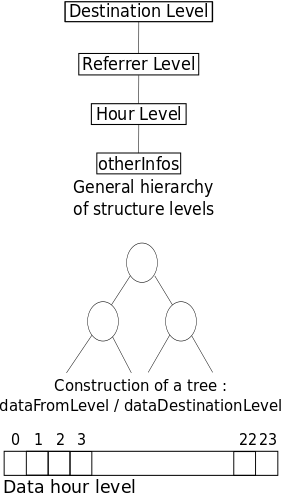
\includegraphics{schemas structures.png}
\end{figure}

\end{document}
